\section{定积分}

\subsection{定积分}

对于 $[a, b]$ 上的函数 $f(x)$,假设我们要求 $y = f(x),\ x = a,\ x = b,\ y = 0$ 围成的曲边梯形的面积,我们可以考虑使用多个小矩形进行近似。

\begin{figure}[htbp]
	\centering
	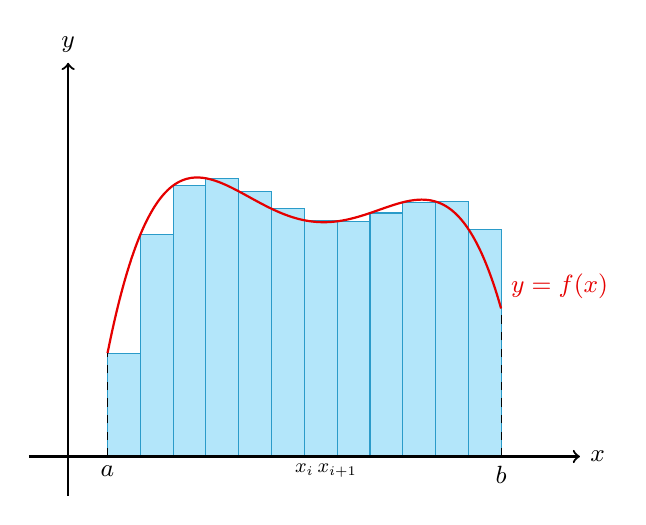
\begin{tikzpicture}[font=\small]
		% ==================================================
		% 1. 参数设置 (在这里修改)
		% ==================================================
		% 定义函数 f(x)
		% 注意:TikZ 的数学语法,乘号不能省,指数用 ^
		\def\func(#1){-0.1 * (#1 - 1) * (#1 - 3) * (#1 - 3.5) * (#1 - 5) + 3}

		% 定义区间 [a, b]
		\def\startx{0.5} % a
		\def\endx{5.5}   % b

		% 定义矩形数量 n
		\def\rectCount{12}

		% 绘图外观设置
		\def\rectColor{cyan!30}       % 矩形填充色
		\def\rectBorder{cyan!80!black}% 矩形边框色
		\def\curveColor{red!90!black} % 曲线颜色
		% ==================================================

		% 2. 自动计算步长 dx
		\pgfmathsetmacro{\dx}{(\endx-\startx)/\rectCount}

		% 4. 绘制矩形 (循环)
		% logic: 循环 i 从 0 到 n-1
		\foreach \i in {0,...,\numexpr\rectCount-1} {
			% 计算当前矩形的左端点 x
			\pgfmathsetmacro{\x}{\startx + \i*\dx}
			% 计算高度 y = f(x)
			\pgfmathsetmacro{\y}{\func(\x)}

			% 绘制矩形:从 (x,0) 画到 (x+dx, y)
			\draw[fill=\rectColor, draw=\rectBorder]
				(\x, 0) rectangle ++(\dx, \y);
		}

		% 3. 绘制坐标轴
		\draw[->, thick] (-0.5, 0) -- (\endx+1, 0) node[right] {$x$};
		\draw[->, thick] (0, -0.5) -- (0, 5) node[above] {$y$};

		% 5. 绘制平滑曲线
		% samples 越高曲线越平滑
		\draw[thick, \curveColor] plot[domain=\startx:\endx, samples=100, smooth] (\x, {\func(\x)});

		% 6. 标注关键点 (可选)
		% 标注 a 和 b
		\draw[dashed] (\startx, 0) -- (\startx, {\func(\startx)});
		\draw[dashed] (\endx, 0) -- (\endx, {\func(\endx)});

		\node[below] at (\startx, 0) {$a$};
		\node[below] at (\endx, 0) {$b$};

		% 标注第 i 个矩形 (示例)
		% 取中间的一个矩形做标注,避免文字重叠
		\pgfmathsetmacro{\midIdx}{int(\rectCount/2)}
		\pgfmathsetmacro{\xMid}{\startx + \midIdx*\dx}
		\node[below, scale=0.8] at (\xMid, 0) {$x_i$};
		\node[below, scale=0.8] at (\xMid+\dx, 0) {$x_{i+1}$};

		% 标注函数名
		\node[above right, \curveColor] at (\endx, {\func(\endx)}) {$y=f(x)$};

	\end{tikzpicture}
	\caption{矩形近似曲边梯形面积}
\end{figure}

假设将 $[a, b]$ 划分为 $n$ 个区间 $[x_i, x_{i+1}]$,第 $i$ 个区间宽度为 $\Delta x_i$,那么面积为

$$
A = \sum_{i=1}^n f(x_i) \Delta x_i
$$

那么当矩形宽度越来越小,面积的极限就是曲边梯形的实际面积。即,若 $\lambda = \max_{i=1}^n \{\Delta x_i\}$,那么:

$$
A = \lim_{\lambda \to 0} \sum_{i=1}^n f(x_i) \Delta x_i
$$

而不管区间的分法如何,$\lambda \to 0$ 时该极限的值是相同的,于是我们可以定义定积分:

\begin{definition}
	设 $f(x)$ 是 $[a, b]$ 上的函数,$A$ 是一个确定的实数。

	若任意 $\varepsilon > 0$,总存在 $\delta > 0$,使得任意 $[a, b]$ 的划分 $T = \{\Delta_i\}_{i=1}^n$ 和 $\xi_i \in \Delta_i$,只要 $\max_{i=1}^n |x| \le \delta$,就有:
	$$
	\left|\sum_{i=1}^n f(\xi_i) |\Delta_i| - A\right| < \varepsilon
	$$
	那么就称 $A$ 为 $f(x)$ 在 $[a, b]$ 上的\textbf{定积分}或 \textbf{Riemann 积分},记作:
	$$
	A = \int_a^b f(x) \dd x
	$$
	此时称 $f(x)$ 在 $[a, b]$ 上 \textbf{Riemann 可积}。

	注意,定义定积分时允许 $a > b$,此时认为 $|\Delta_i| < 0$。
\end{definition}

那么可以自然得到定积分的几何意义就是 $f(x)$ 在 $[a, b]$ 上与 $x$ 轴围出的有向面积。

\begin{example}
	证明 Diriclet 函数 $D(x) = [x \in \mathbb{Q}]$ Riemann 不可积。

	\begin{proof}
		对于一个划分 $T$,先取 $\xi_i \in \mathbb{Q}$,那么:
		$$
		A_1 = \sum_{i=1}^n f(\xi_i) |\Delta x_i| = \sum_{i=1}^n 1 \cdot |\Delta_i| = 1
		$$
		再取 $\xi_i \notin \mathbb{Q}$,那么:
		$$
		A_2 = \sum_{i=1}^n f(\xi_i) |\Delta x_i| = \sum_{i=1}^n 0 \cdot |\Delta_i| = 0
		$$
		于是 $A_1 \neq A_2$,极限不存在。
	\end{proof}
\end{example}

\subsection{可积的条件}

首先可以给出一个必要条件:

\begin{theorem}
	若 $f(x)$ 在 $[a, b]$ 上可积,那么它在 $[a, b]$ 上有界。

	\begin{proof}
		假设 $f(x)$ 在 $[a, b]$ 上无解,那么 $[a, b]$ 的任意一个划分 $T$ 必然存在一个子区间 $\Delta_k$ 使得 $f(x)$ 在 $\Delta_k$ 上无界。那么
		$$
		\forall\,A > 0: \exists\,\xi_k \in \Delta_k: |f(\xi_k)| > \frac{A}{|\Delta_k|}
		$$
		那么,取定所有 $i \neq k$ 的 $\xi_i$ 后,有:
		$$
		\left| \sum_{i=1}^n f(\xi_i) |\Delta_i| \right| \ge A - \left|\sum_{i \neq k} f(\xi_i) |\Delta_i| \right| 
		$$
		于是这是一个无界的量,极限是不存在的。
	\end{proof}
\end{theorem}

在此基础上,再进一步探讨更强的条件:

\begin{definition}[Darboux 上和与 Darboux 下和]
	设 $f(x)$ 在 $[a, b]$ 有界,取 $[a, b]$ 的划分 $T: x_0 = a < x_1 < x_2 < \cdots < x_n = b$,记 $m_i \inf\limits_{x \in [x_{i-1}, x_i]} f(x),\ M_i = \sup\limits_{x \in [x_{i-1}, x_i]} f(x)$,定义和式:

	\begin{itemize}
		\item Darboux 上和:$\displaystyle S(T, f) = \sum_{i=1}^n M_i (x_i - x_{i-1})$;
		\item Darboux 下和:$\displaystyle s(T, f) = \sum_{i=1}^n m_i (x_i - x_{i-1})$。
	\end{itemize}
\end{definition}

\begin{theorem}
	设 $f(x)$ 在 $[a, b]$ 有界,且有两个划分 $T, T'$,满足 $T'$ 是 $T$ 的更细划分,那么:
	$$
	S(T, f) \ge S(T, f),\ s(T, f) \le s(T', f)
	$$
\end{theorem}

\begin{definition}
	设 $f(x)$ 在 $[a, b]$ 上有界,$T$ 为 $[a, b]$ 的任意划分。那么定义:
	$$
	\overline{I} = \inf S(T, f),\ \underline{I} = \sup s(T, f)
	$$
	其中 $\overline{I}$ 称为 $f(x)$ 在 $[a, b]$ 上的\textbf{上积分},$\underline{I}$ 称为 $f(x)$ 在 $[a, b]$ 上的\textbf{下积分}。
\end{definition}

\begin{theorem}
	设 $f(x)$ 在 $[a, b]$ 上有界,那么下面的命题等价:

	\begin{itemize}
		\item $f(x)$ 在 $[a, b]$ 可积;
		\item $\overline{I} = \underline{I}$;
		\item 对于任意 $[a, b]$ 的划分 $T$,有 $\displaystyle \lim\limits_{\lVert T \rVert \to 0} \sum_{i=1}^n \omega_i |\Delta_i| = 0$,其中 $\omega_i = M_i - m_i$;
		\item 对于任意 $\varepsilon > 0$,总存在划分 $T$,使得 $\displaystyle \sum_{i=1}^n \omega_i |\Delta_i| < \varepsilon$。
	\end{itemize}
\end{theorem}

此外,可以给出一些可积的函数类别:

\begin{theorem}
	若 $f(x)$ 在 $[a, b]$ 上连续,那么 $f(x)$ 在 $[a, b]$ 上可积。

	\begin{proof}
		$f(x)$ 在 $[a, b]$ 上连续,那么也一致连续,因此:
		$$
		\forall\,\varepsilon > 0: \exists\,\delta > 0: \forall\,x_1, x_2 \in [a, b], |x_1 - x_2| < \delta: |f(x_1) - f(x_2)| < \frac{\varepsilon}{b - a}
		$$
		那么对于 $[a, b]$ 的任意划分 $T$,当 $\lVert T \rVert < \delta$ 时,有:
		$$
		\sum_{i=1}^n \omega_i |\Delta_i| = \sum_{i=1}^n (f(s_i) - f(t_i)) |\Delta_i| < \sum_{i=1}^n \frac{\varepsilon}{b - a} |\Delta_i| < \varepsilon
		$$
		于是得证。
	\end{proof}
\end{theorem}

\begin{corollary}
	若 $f(x)$ 在 $[a, b]$ 上是有有限个间断点的有界函数,那么 $f(x)$ 在 $[a, b]$ 上可积。
\end{corollary}

\subsection{定积分的性质}

\begin{property}[定积分的线性性]
	设 $f(x), g(x)$ 在 $[a, b]$ 可积,$\alpha, \beta \in \mathbb{R}$,那么:
	$$
	\int_a^b \ab(\alpha f(x) + \beta g(x)) \dd x = \alpha \int_a^b f(x) \dd x + \beta \int_a^b g(x) \dd x
	$$
\end{property}

\begin{property}[定积分的保号性]
	若 $f(x)$ 在区间 $[a, b]\ (a < b)$ 上可积且非负,那么:
	$$
	\int_a^b f(x) \dd x \ge 0
	$$
\end{property}

\begin{property}[估值不等式]
	若 $f(x)$ 在区间 $[a, b]$ 上可积,且 $m \le f(x) \le M$,那么
	$$
	m(b - a) \le \int_a^b f(x) \dd x \le M(b - a)
	$$
\end{property}

\begin{property}[积分区间可加性]
	$f(x)$ 在 $[a, b]$ 可积 $\Leftrightarrow$ 任意 $c \in [a, b]$,$f(x)$ 在 $[a, c], [c, b]$ 上也可积,并且
	$$
	\int_a^b f(x) \dd x = \int_a^c f(x) \dd x + \int_c^b f(x) \dd x
	$$
	\begin{proof}
		根据 $[a, b]$ 上可积,可知对任意 $\varepsilon > 0$ 存在划分 $T$ 使得 $\lVert T \rVert \to 0$ 时 $\sum_{i=1}^n \omega_i |\Delta_i| < \varepsilon$。那么给 $T$ 增加一个分割点 $c$ 得到新的划分 $T^*$,因为上和不增、下和不减,因此:
		$$
		\sum_{i=1}^{n+1} \omega^*_i |\Delta^*_i| \le \sum_{i=1}^n \omega_i |\Delta_i| < \varepsilon
		$$
		而 $T^*$ 也可以分成 $[a, c], [c, b]$ 上的划分 $T_1, T_2$,因此 $f(x)$ 在 $[a, c], [c, b]$ 也可积。反之亦可以类似证明。

		下面再证明 $\int_a^b f(x) \dd x = \int_a^c f(x) \dd x + \int_c^b f(x) \dd x$。

		\begin{itemize}
			\item 若 $c \in [a, b]$:此时可以取 $c$ 为第 $k$ 个分割点,那么:
			$$
			\begin{aligned}
				\int_a^b f(x) \dd x & = \lim_{\lambda \to 0} \sum_{i=1}^n f(\xi_i) |\Delta_i| \\
				& = \lim_{\lambda \to 0} \sum_{i=1}^k f(\xi_i) |\Delta_i| + \lim_{\lambda \to 0} \sum_{i=k+1}^n f(\xi_i) |\Delta_i| \\
				& = \int_a^c f(x) \dd x + \int_c^b f(x) \dd x
			\end{aligned}
			$$

			\item 若 $c \notin [a, b]$,不妨设 $c > b > a$,那么:
			$$
			\begin{aligned}
				\int_a^c f(x) \dd x & = \int_a^b f(x) \dd x + \int_b^c f(x) \dd x \\
				\int_a^b f(x) \dd x & = \int_a^c f(x) \dd x - \int_b^c f(x) \dd x \\
				& = \int_a^c f(x) \dd x + \int_c^b f(x) \dd x
			\end{aligned}
			$$
		\end{itemize}
	\end{proof}
\end{property}